\documentclass{article}
\usepackage[utf8]{inputenc}
%\usepackage [danish]{babel} % Vi burde ikke have brug for den her
\usepackage[a4paper, hmargin={2.8cm, 2.8cm}, vmargin={2.5cm, 2.5cm}]{geometry}
\usepackage{eso-pic} % \AddToShipoutPicture
\usepackage{graphicx} % \includegraphics
\usepackage{wrapfig, blindtext}
\usepackage{array}
\usepackage{import}
\usepackage[hidelinks]{hyperref}
\usepackage{verbatim}
\usepackage{algorithm}
\usepackage{float}
\linespread{1.2}
\usepackage{pbox}
\usepackage{amsthm}
\usepackage{mathtools}
\usepackage{amsmath}
\usepackage{url}
\usepackage{listings}
\usepackage{tikz}
\usetikzlibrary{arrows,automata,fit}
\usepackage{amsfonts}
\usepackage{standalone}
\newtheorem{theorem}{Teorem}
\newtheorem{lemma}{Lemma}
\newtheorem{korollar}{Korollar}
\newcolumntype{L}[1]{>{\raggedright\let\newline\\\arraybackslash\hspace{0pt}}m{#1}}
\newcolumntype{C}[1]{>{\centering\let\newline\\\arraybackslash\hspace{0pt}}m{#1}}
\newcolumntype{R}[1]{>{\raggedleft\let\newline\\\arraybackslash\hspace{0pt}}m{#1}}

\newcommand*\Let[2]{\State #1 $\gets$ #2}
\usepackage[noend]{algpseudocode}

\usepackage{algorithmicx}

\newtheorem{mydef}{Definition}
\newtheorem{myex}{Example}[section]
\usepackage{caption}
\DeclareMathOperator*{\argmin}{arg\,min}

\author{
\huge{Supervisors}\\
\Large{Rasmus Fonseca}\\
\Large{Niels Bjørn Bugge Grathwohl}\\
\Large{Ulrik Rasmussen}\\
\Large{Martin Asser Hansen}\\
    \\ \texttt{}
}

\title{
  \vspace{3cm}
  \Huge{Genome pattern matching using regular expressions} \\
  \Large{Simon Nicolai Lefoli Maibom - xvm226} \\
  \Large{Arinbjörn Brandsson - hkt789}\\
  \Large{Martin Simon Haugaard - cdl966}
}

\usepackage{natbib}
\usepackage{graphicx}

\newcommand{\myfl}{\left\lfloor}
\newcommand{\myfr}{\right\rfloor}
\newcommand{\mycl}{\left\lceil}
\newcommand{\mycr}{\right\rceil}

\begin{document}

%% Change `ku-farve` to `nat-farve` to use SCIENCE's old colors or
%% `natbio-farve` to use SCIENCE's new colors and logo.
\AddToShipoutPicture*{\put(0,0){\includegraphics*[viewport=0 0 700 600]{lib/natbio-farve}}}
\AddToShipoutPicture*{\put(0,602){\includegraphics*[viewport=0 600 700 1600]{lib/natbio-farve}}}

%% Change `ku-en` to `nat-en` to use the `Faculty of Science` header
\AddToShipoutPicture*{\put(0,0){\includegraphics*{lib/nat-en}}}

\clearpage\maketitle
\thispagestyle{empty}

\newpage
\begin{abstract}
%insert abstract
\end{abstract}
\newpage
\tableofcontents
 
\newpage

%\section{Introduction}
\section{Introduction}%Probably write some about what we did, and 
%What our result(s) were?
When the Human Genome Project~\cite{hgp} (a project which had the goal of sequencing 
all 22 chromosomes of the human genome) was launched in 1990, the project was 
budgeted to cost 3 billion dollars and was estimated to take fifteen years 
to complete. However as technology progressed, the project managed to complete 
its goal two years earlier than expected, in 2003. This was made possible 
because of the rapid advancements in genome sequencing, and the advancement 
has not stopped since. This has led to decreasing costs of sequencing RNA and DNA, 
meaning biologists has access to greater amounts of data than before. 
However the technology to process these amounts of data have not progressed at 
the same pace as sequencing. Scan\_for\_matches is a tool for pattern-matching, 
which searches through data files to match a pattern specified by a user. 
While scan\_for\_matches has proven to be a fast and reliable 
tool, due to the amount of data it shifts through, a faster alternative 
is desired.\\\\
In this thesis, we provide an alternative to scan\_for\_matches based on 
automata theory and regular expressions. While the implementation currently 
does not match scan\_for\_matches' speed, with optimization it could. We will 
discuss the implementation's strengths and weaknesses, and describe what 
future work with the implementation will involve.
Our implementation can be found at 
"\url{https://github.com/smaibom/bach_2015/tree/master/Implementation/src}".
\begin{comment}
After hearing about this problem, we thought that there must be a better 
way of searching through data that is also theoretically sound. Our first 
thought was using automata-based searching methods, since this provides a 
calculable best- and worst-case run time while being theoretically sound. 
Since regular expressions uses an automata-based way of searching, we hypothesized 
that implementing regular expressions which have the same functions as 
scan\_for\_matches would lead to faster run times.
\end{comment}

\section{Problem Analysis}\label{probanal}
%INTRODUCTION TO PROBLEM ANALYSIS
The functionality of scan\_for\_matches dictates what our solution must be able to do. While a more indepth analysis of the functionality 
of scan\_for\_matches can be found in section~\ref{scanformatches}, 
the requirements for our solution are as follows:
\begin{enumerate}
\item Read a data file
\item Match
\begin{enumerate}
\item with errors allowed
\item a previously found match
\item a modified pattern
\end{enumerate}
\item Return matches with their position
\end{enumerate}
While some of the functionality (items 1 and 3) will be trivial to implement 
since they are standard functions of most programming languages, there are 
some challenges to be found in regards of what we must match. Matching with 
errors allowed are not supported natively in regular expressions, and 
matching a modified text, which may first be determined at runtime, will be 
challenging to implement with automata.

\section{State-of-the-Art}
 \subsection{KMC}
 %Mangler noget her
 \subsection{RE2} %Google's RE engine
 RE2 is Google's regular expression engine written in C++. It supports 
 backtracking, but not backreferencing since backreferencing can't be implemented 
 efficiently according to~\cite{web6}. Since RE2 doesn't support matching with 
 errors or backreferencing, it would be unable to properly reproduce 
 scan\_for\_matches' functionality.
 
 \subsection{TRE} %Got both backtracking and backreferencing
 TRE was created by Ville Laurikari for his master's thesis in 2001, and 
 is a regular expression engine supporting backtracking, backreferencing and 
 matching with errors. Because of this, TRE is the best candidate for modification 
 in order to make it work with patterns. We expand on this in section~\ref{tre}.

%\newpage

%\section{Preliminaries}
\section{Deoxyribonucleic and Ribonucleic Acids}
Deoxyribonucleic acids (DNA) and ribonucleic acids (RNA), collectively known as 
nucleic acids, are one of the three 
essential molecules for life, the last two being proteins and carbohydrates. 
DNA creates RNA through transcription and RNA creates proteins through 
translation, while proteins performs a variety of tasks, one 
of which is packaging and controlling the long DNA molecules~\cite[p. 172]{alberts}. 
In this section we will briefly detail the functions of DNA and RNA as well as their 
secondary structure.
\subsection{DNA}
Deoxyribonucleic acid (DNA) is a macro molecule composed of nitrogenous bases 
joined by deoxyribose-phosphate into long strands. One nitrogenous base which 
is joined with a sugar\footnote{Deoxyribose or ribose}-phosphate is called a 
nucleotide. DNA can have four nitrogenous bases:
\begin{itemize}
\item Guanine (G)
\item Adenine (A)
\item Cytosine (C)
\item Thymine (T)
\end{itemize}
DNA is primarily found in nature as helixes, where two strands have bonded. Each 
base has a complementary base with which they can form a hydrogen bond. 
G is the complementary base of C and A is the complementary base of T.

DNA holds the hereditary material of the cells and can replicate itself by 
detaching two bonded strands, then use each as a template for a new strand 
to bond with the detached strands~\cite[p. 199]{alberts}.
\subsection{RNA}
Ribonucleic acid (RNA) is a macro molecule composed of long strands of 
nucleotides. RNA have the same nitrogenous bases as DNA except for T, which is 
changed during transcription from DNA to RNA into Uracil (U) which bonds with 
A. In nature, the predominant form of RNA are as single-stranded chains that 
can fold back on themselves or bundled with other chains to form a structure. This 
flexibility of the backbone, which allows for chains to fold in on themselves is 
possible because the RNA's backbone is composed of a sugar called ribose, which 
allows more flexibility compared to its alternative form, deoxyribose, used in 
deoxyribonucleic acid (DNA).

%Maybe delete next part
When DNA creates RNA through transcribing portions of its sequence\footnote{A 
sequence is a succession of nucleotides}, five different kinds of RNA are 
created. Three are responsible for protein synthesis which allows for the creaiton 
of proteins, one is for regulating the DNA's gene expression, and the last 
is used for miscellaneous functions\cite[p. 236, table 7-1]{alberts}.
\subsection{Secondary Structure}\label{structs}
The secondary structure of DNA and RNA describes how bases of 
strands bond to themselves. The secondary structure can change if 
a strand is damaged or has mutated, causing it to gain or lose 
bases. Below are examples of three common secondary structures.

\subsubsection{Bulge}
A bulge occurs when one or more bases have no base to bond with, and these 
bases are surrounded by bases which have bonded. This causes the bases to get 
pushed out slightly, resembling a bulging growth. This type of structure occurs 
when one or more bases has been inserted or deleted. If a base has been 
inserted it will have no base to bond with, and if a base has been deleted 
the previously-bonded base will have no base to bond with. Figure~\ref{fig:bulge} shows a bulge.

\begin{figure}[H]
\centering
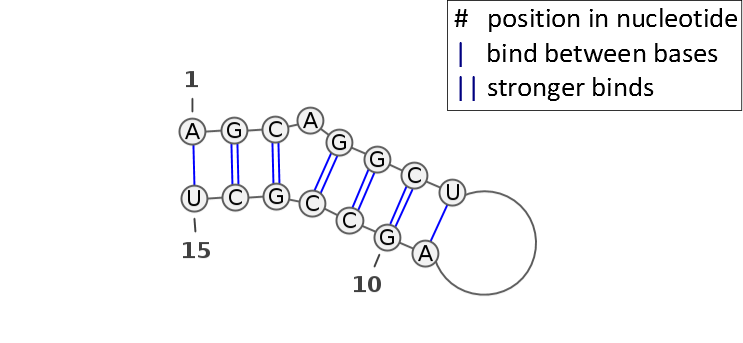
\includegraphics[scale=0.4]{./lib/bulge.png}
\caption{The RNA sequence {\tt AGCAGGCUAGCCGCU}. Note the bulging {\tt A} at position 4.}
\label{fig:bulge}
\end{figure}~
\\
\subsubsection{Interior Loop}
An interior loop occurs when two or more opposing bases are not complementary and 
can not bond, causing them both to bulge. This occurs when one or more 
consecutive bases mutate to another base. Figure~\ref{fig:int-loop} shows an interior 
loop.
\begin{figure}[h!]
\centering
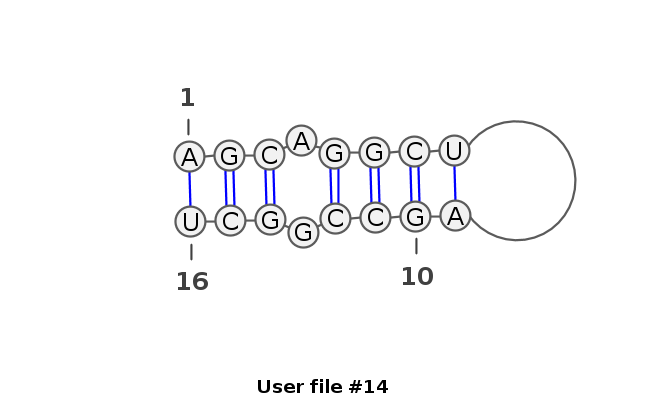
\includegraphics[scale=0.4]{./lib/interior-loop.png}
\caption{The RNA sequence {\tt AGCAGGCUAGCCGGCU}. Note the bulging {\tt A} at position 4 and {\tt G} at position 13
creating a loop inside the bonded strand.}
\label{fig:int-loop}
\end{figure}\\
These interior loops vary in size, and can have differing amount of bases on 
either side of the strands.
\subsubsection{Stem Loop}
A stem loop, also known as a hairpin loop, occurs when a strand bonds with 
itself, but leaves a sequence of bases sticking out, which does not bond with anything. 
This kind of loop occurs typically in RNA as they are single-stranded, but may 
happen in single stranded DNA. Figure~\ref{fig:stem-loop} 
shows a stem loop.
\begin{figure}[h!]\centering
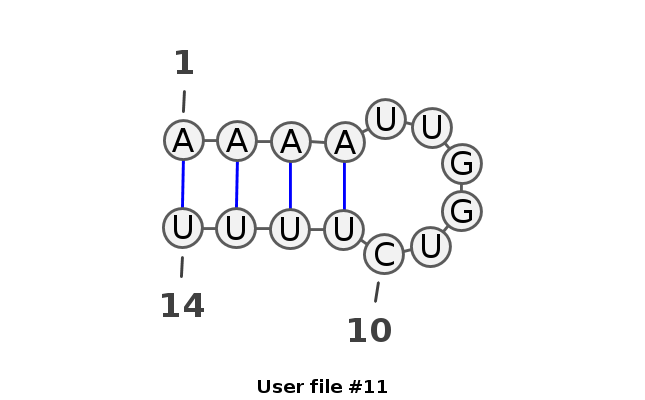
\includegraphics[scale=0.35]{./lib/stem-loop.png}
\caption{A stem loop of the RNA sequence {\tt AAAAUUGGUCUUUU}.}
\label{fig:stem-loop}
\end{figure}\\
An important thing to note is how the sequence can be seen as one 
long strand that starts from the adenine bases, which binds with the uracil bases, 
loops around without binding to anything and finally become the uracil bases 
which binds with the adenine bases from the beginning. This means that the 
stem loop from Figure~\ref{fig:stem-loop} can be written as one continuous 
sequence of bases; {\tt AAAAUUGGUCUUUU}. Since we can define a stem loop, we can 
search through a file documenting the bases of a nucleic acid and find all stem 
loops.

%\section{Theory}
\newpage
\section{Regular expressions} 
  To explain what a regular expression is, we must first introduce languages and alphabets. All literals will be written using the typewriter font, to distinguish 
\begin{mydef}\label{alph}
An alphabet $\Sigma$ is a finite set of letters.
\end{mydef}

\begin{mydef}\label{lang}
A language is a infinite set of strings, composed by letters from an alphabet $\Sigma$
\end{mydef}

\begin{myex}
If we have a DNA sequence string, the alphabet $\Sigma$ consists of the literals ${\tt\{t,g,c,a\}}$. and the language contains strings formed by the literals from this alphabet. For example "gtcaaa" or "gtcaaat". 
\end{myex}

\begin{mydef}
E is a regular expression(RE) if either:
\begin{itemize} 
\item E is a atomic expression, that consist of a letter from an alphabet $\Sigma$ or special character 1.
\item Given two RE's $E_1$ and $E_2$. E is a compound expression formed by $E_1 + E_2$, $E_1 E_2$ or $E_1 ^*$ 
\end{itemize}
\end{mydef}



\begin{mydef}
A regular expression is described by the following grammar: \\
\begin{center}
$E::= a|1|E_1 + E_2 |E_1 E_2 | E^* | 0$
\end{center}
where $E_1$ and $E_2$ are RE's and $a \in \Sigma$
\end{mydef}

\begin{mydef}\centering
The language interpation of L(E) of a regular expression is: 
\begin{align*}
L(0)           &= \emptyset\\
L({\tt a})     &= \{{\tt a}\} \\
L(1)         &= \{\epsilon\} \\
L(E_0 + E_1) &= L(E_0) \cup L(E_1) \\
L(E_1 E_2)   &= \{w_1w_2 | w_1 \in L(E_1),w_2 \in L(E_2)\}=L(E_1)L(E_2) \\
L(E^*)       &= \bigcup\limits_{n=0}^\infty L(E)^n 
\end{align*}
%\cite[p.5 def. 3]{crash}
\end{mydef}

With definition 2, we can now form regular languages. For example, natural numbers described as a regular expression. Natural numbers have the alphabet $\Sigma$ = \{{\tt 0,1,2,3,4,5,6,7,8,9}\}, the regular expression for natural numbers would look like:
\begin{center}
$E_{nat} = $(1+2+3+4+5+6+7+8+9)(0+1+2+3+4+5+6+7+8+9)$^*$
\end{center}

\newpage

\section{Nondeterministic Finite Automaton}
\begin{mydef}
An nondeterministic finite automaton (NFA) is a 5-tuple $(Q,\Sigma,\Delta,q^s ,q^f)$. Where $Q$ is a finite set of states,$\Sigma$ is the input alphabet, the initial state $q^s \in Q$,  the accepting state $q^f \in Q$ and $\Delta$ is the set that contains all the transitions. Transitions in $\Delta$ is shown $q^1\xrightarrow{a}q^2$ where $q^1\in Q,q^2\in Q$ and the label $a$ is either $a \in \Sigma$ or  the empty transition $\epsilon$
\end{mydef}

\subsection{Conversion from RE to NFA}
\label{RA_TO_NFA}
One of the main reasons for using NFAs when working with regular expressions is the direct correlation between regular expressions and NFAs. Each expression can be converted to an NFA, and vice versa. Table~\ref{tab:NFA_TAB} shows the correlation between regular expressions and NFA for the most common expressions.
%\\
%(( NOTE: We'll include a table with conversions ))
%\\
%With little effort every regular expression can be translated into a graph, which can then be analysed.

\begin{table}[h!]
\caption{Translation table from regular expressions to NFA}
\centering
\begin{tabular}{*{2}{m{0.4\textwidth}}}
\hline
\begin{center}$a$\end{center} &\begin{center} 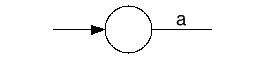
\includegraphics[width=0.25\textwidth]{lib/dot/a.png} \end{center} \\
\hline
\begin{center}$\epsilon$\end{center} &\begin{center} 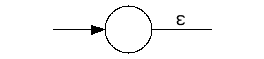
\includegraphics[width=0.25\textwidth]{lib/dot/epsilon.png} \end{center} \\
\hline
\begin{center}$ab$\end{center} &\begin{center} 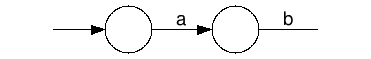
\includegraphics[width=0.3\textwidth]{lib/dot/ab.png} \end{center} \\
\hline
\begin{center}$a\vert b$\end{center} &\begin{center} 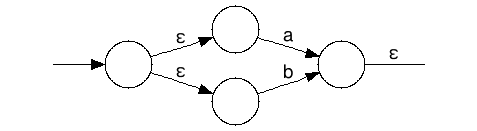
\includegraphics[width=0.35\textwidth]{lib/dot/a-or-b.png} \end{center} \\
\hline
\begin{center}$a^*$\end{center} &\begin{center} 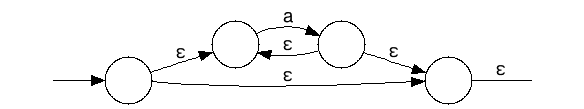
\includegraphics[width=0.4\textwidth]{lib/dot/a_star.png} \end{center} \\
\hline
\end{tabular}
\label{tab:NFA_TAB}
\end{table}

%
%\begin{figure}[h!]
 % \centering
%\begin{minipage}[b]{0.40\linewidth}
 % \centering
   %   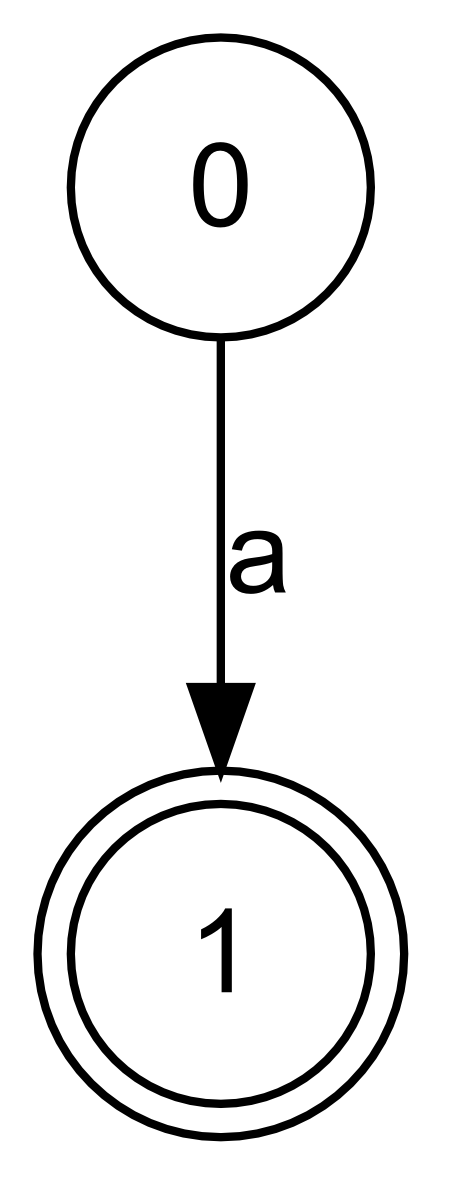
\includegraphics[width=0.2\textwidth]{lib/A.png}
  %\caption{NFA of the expression $a$}
%\label{fig:A}
%  \end{minipage}
%\begin{minipage}[b]{0.40\linewidth}

%  \centering
   %   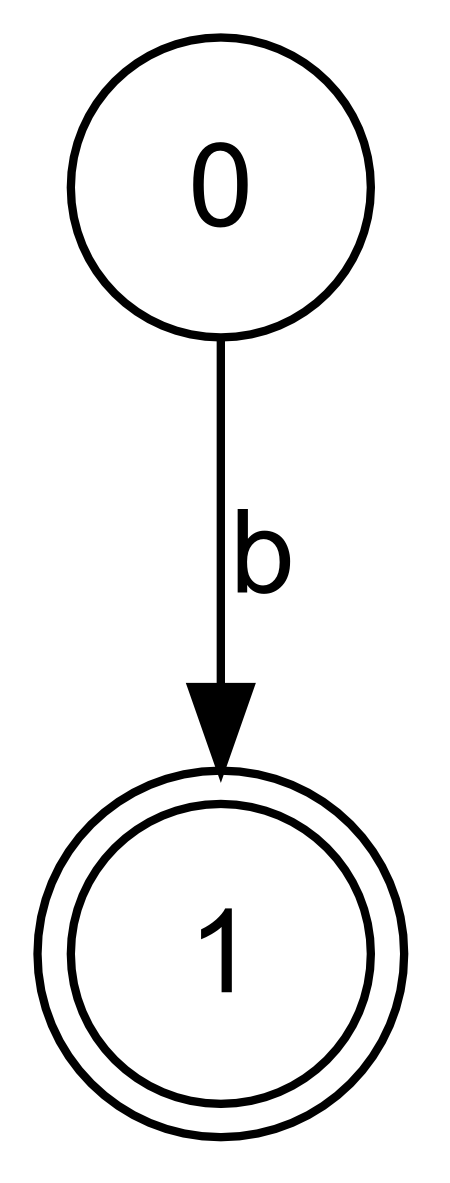
\includegraphics[width=0.2\textwidth]{lib/B.png}
  %\caption{NFA of the expression $b$}
  %\label{fig:B}
%    \end{minipage}
%\end{figure}

%For example two NFAs of regular expression $a$ and $b$ will appear as shown in Figure~\ref{fig:A} \& \ref{fig:B}, each of them starts in node $0$ and ends in node $1$, and these nodes are connected by a one-way transition with a value $a$ or $b$. %, it may be worth noting that our implementation always converts to lower case when constructing and matching.

%To construct the NFA for $A | B$ , one will first have to construct an NFA for both $A$ and $B$, which will then be combined, making the full NFA. The $|$ operator this is achieved by constructing two new nodes, the first having epsilon-transition pointing to the start node of each of the two NFAs $A$ and $B$, then for each NFA $A$ and $B$ the ending node will instead of ending the NFA, have a new epsilon-transition to the second new node, in the figure below, Figure~\ref{fig:A_OR_B}, the two new nodes are labeled $0$ and $5$:

%\begin{figure}[h!]
 % \centering
   %   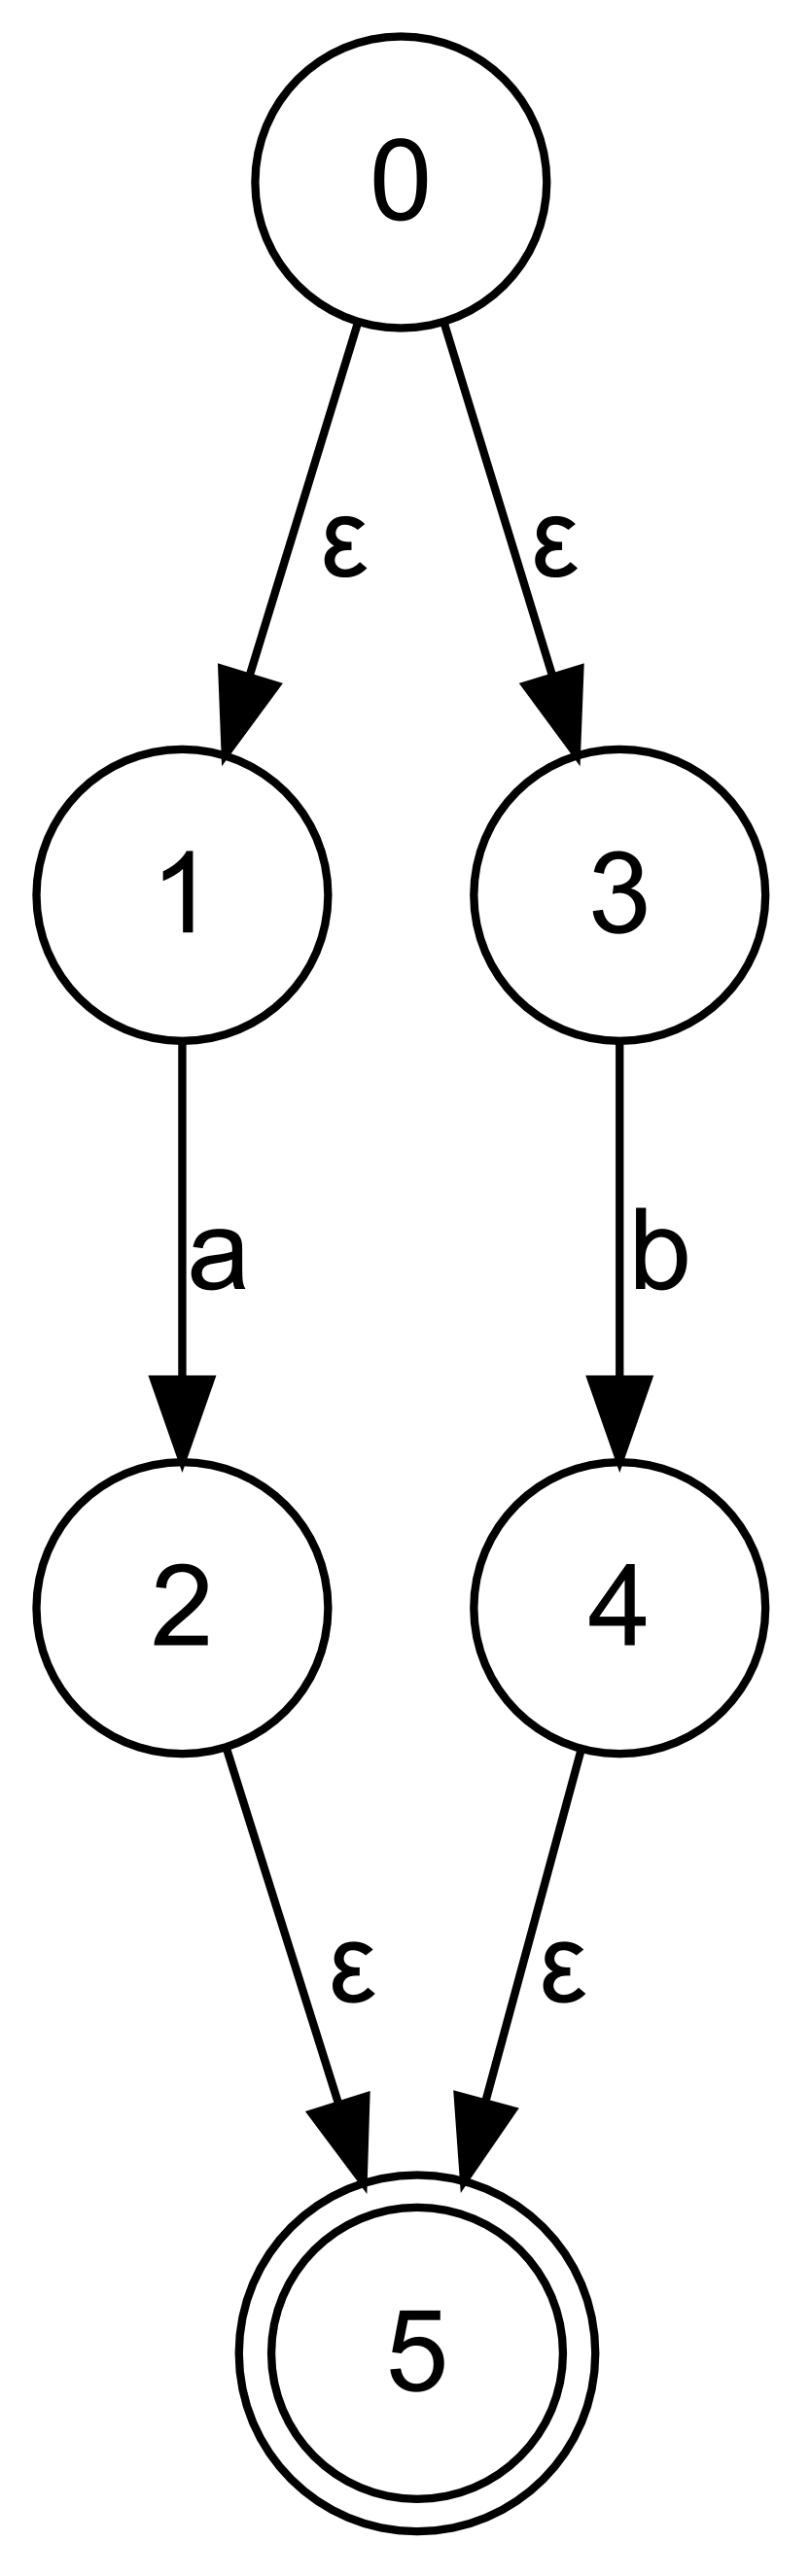
\includegraphics[width=0.1\textwidth]{lib/A_OR_B.png}
 % \caption{NFA of the expression $a | b$}
%\label{fig:A_OR_B}
%\end{figure}

Once a NFA-structure has been build, we can start matching a text against the NFA.

This is achieved by having a set of states, each state is looking at a node in the structure, while keeping track of previous nodes traversed by the state. Whenever a new character is being checked to match, each state will look at its node, and determine if it's possible to accept the character in the NFA, either by taking a transition labeled with the character, or alternatively via an epsilon-transition. When two possible transitions are viable, new states will be created in the set of states, so that each possible transition will be explored.

Any state that will fail to match the character will be removed from the set of states.
%\begin{figure}[h!]
 % \centering
%\begin{minipage}[b]{0.40\linewidth}
 % \centering
   %   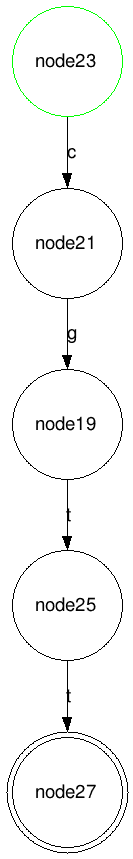
\includegraphics[width=0.2\textwidth]{lib/cgtt1.png}
   % \caption{NFA of $CGTT$, with a state looking at node23.\\}
    %\label{fig:CGTT_1}
 % \end{minipage}
%\begin{minipage}[b]{0.40\linewidth}
%\centering
%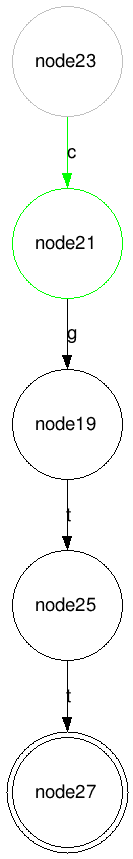
\includegraphics[width=0.2\textwidth]{lib/cgtt2.png}
% \caption{Next iteration of the state on Figure~\ref{fig:CGTT_1}, the state is now in node21.}
  %  \end{minipage}
%\label{fig::cgtt}
%\end{figure}

Only if a state reaches the ending node of the NFA, there's a match.

\newpage

\subsection{Insertions, Deletions and Mutations}
NFAs do not support mismatching by default, although a regular expression can be built to handle mismatches. While doing handling mismatching while constructing the regular expression, we are interested in having an NFA, and allowing matching while with support for insertions, deletions and mutations, hence we need to define a way to handle this.

We can do this by adding a counter for insertions, deletions and mutations, and when a transition is not possible in the NFA, we decrease these counters and preform alternative transitions to emulate these conditions.
%Currently our implementation supports a simple solution to the insertion, deletion and mutation problem, which is achieved by having a counter for insertions, deletions and mutation in each state, these counters symbolise the number of allowed occurrences of each mutation, insertion and deletion.
\begin{description}
\item[] For insertions, the state will remember the unmatched character, but the state won't move from its current node.
\item[]For deletions, the state wont remember the unmatched character, but it will take every transition going on from the node.
\item[] For mutations, the same happens as in a deletion, but now the state also remembers the unmatched character.
\end{description}
Figure~\ref{fig:ins_mut_del} illustrates how states move through a NFA when mismatches occur. 

\begin{figure}[h!]
  \centering
      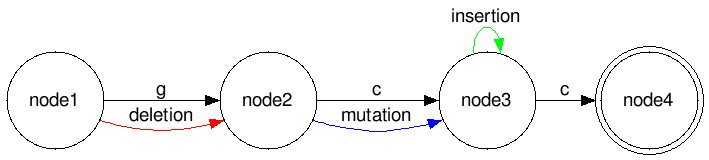
\includegraphics[width=0.6\textwidth]{lib/gcc_ins_mut_del.png}
  \caption{Simple NFA of $GCC$, showing behaviour of insertion, mutation and deletion}
\label{fig:ins_mut_del}
\end{figure}
%Depending on the number of insertions, deletions and mutations allowed, this approach will grant each state a much longer lifespan, and for each non-matching character parsed, one state may turn into three, which all needs to be processed for each new character parsed, resulting in an increasingly slower running time as the allowed number of insertions, deletions and mutations increase, but it does give us the utility that we require.
%\label{state:insertion1}


%In the next iteration of our implementation, we aim to implement levenstein automations\cite{WikiLevenshtein}, which hopefully will help speed up the runtime, and also, currently our solution will work on any given regular expression, thus a logical step which also may deliver some increase in performance would be to enforce a constriction such that it only allows for a RNA language similar to that defined in Section~\ref{section:RE}.
\newpage

\subsection{Matching using NFA}

\begin{algorithm}
  \caption{NFA simulation
    \label{nfasim}}
  \begin{algorithmic}[1]
    \Require{$N$ is a NFA and $x$ is a string}
    \State
    \Function{Simulation}{$N(Q,\Sigma,\Delta,q^s,q^a), x$}
      \Let{$stateset$}{$\{q^s\}$} 
      \For{{\bf each} symbol {\bf in} $x$}
        \If{$stateset = \emptyset$} 
            \State \Return{False}
        \EndIf
        \Let{$next$}{$\emptyset$}
        \Let{$states$}{$\epsilon$-closure($stateset$)}
        \Let{$stateset$}{$next$}
      \EndFor
      \If{$q^a \in stateset$}
        \State \Return{True}
      \EndIf
      \State \Return{False}
    \EndFunction
  \end{algorithmic}
\end{algorithm}
\section{Tagged NFA}
\label{sec:tnfa}
The tagged NFA (\emph{TNFA}) is introduced in \cite{Ville}. It introduces the concept of tagging NFA transitions. A TNFA is a NFA which allows for mismatches in the input string.

\begin{mydef}
A tagged NFA is a 6 tuple $(Q,\Sigma,\Delta,q^s,q^a,\Delta')$ where the first 5 elements is a standard NFA and $\Delta'$ is a set of tuples containing transitions for mismatches. The type of $\Delta'$ is \\$\Delta' \subseteq Q \cdot\{\epsilon\} \cdot Q \cdot M$, where $M = \{i,d,a\}$ for mismatch types.  
\end{mydef}
TNFA adds a new literal construction rule. A new set of tagged $\epsilon$-transitions is added as shown in Tabel \ref{tab:TNFA} on the new literal construction rule. Transitions in $\Delta'$ are represented as $(q,\epsilon,q,i) \in \Delta'$ for insertions,$(q,\epsilon,q',d) \in \Delta'$ for deletions and $(q,\epsilon,q',a) \in \Delta'$ for alterations, we write these transitions as $(q {\color{green} \xrightarrow{{\color{black}\epsilon/i}}} q)$ for insertions, $(q {\color{red} \xrightarrow{{\color{black}\epsilon/d}}} q')$ for deletions and $(q {\color{blue} \xrightarrow{{\color{black}\epsilon/a}}} q')$ for alterations.
\begin{table}[h]\label{nfac}
\caption{Translating table for literal construction of TNFA}
\label{nfac}
\centering
\begin{tabular}{*{2}{m{0.4\textwidth}}}
\hline
\begin{center}$0$\end{center} &\begin{center}
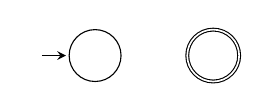
\begin{tikzpicture}[->,>=stealth,shorten >=1pt,auto,node distance=2 cm, scale = 0.75, transform shape,initial text={}]
  \node [initial, state] (0) {};
  \node [accepting,state, right of=0] (1) {};

\end{tikzpicture}\end{center} \\
\hline
\begin{center}$1$\end{center} &\begin{center} 
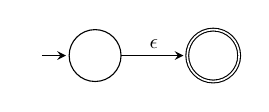
\begin{tikzpicture}[->,>=stealth,shorten >=1pt,auto,node distance=2 cm, scale = 0.75, transform shape,initial text={}]
  \node [initial, state] (0) {};
  \node [accepting,state, right of=0] (1) {};

  \path[->] (0) edge node [above] {$\epsilon$} (1);

\end{tikzpicture} \\
\end{center} \\
\hline
\begin{center}$a$\end{center} &\begin{center}
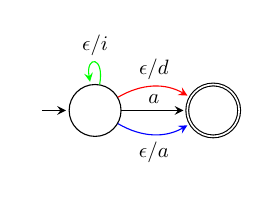
\begin{tikzpicture}[->,>=stealth,shorten >=1pt,auto,node distance=2 cm, scale = 0.75, transform shape,initial text={}]
  \node [initial, state] (0) {};
  \node [accepting,state, right of=0] (1) {};

  \path[->] (0) edge node [above] {$a$} (1);
  \path[->] (0) edge [color=green, in=100,out=80,loop] node [color=black, above] {$\epsilon/i$} (0);
  \path[->] (0) edge [color=red,bend left] node [color=black, above] {$\epsilon/d$} (1);

  \path[->] (0) edge [color=blue,bend right] node [color=black, below] {$\epsilon/a$} (1);
\end{tikzpicture}\end{center}\\
\hline
\begin{center}$E^1E^2$\end{center} &\begin{center} 
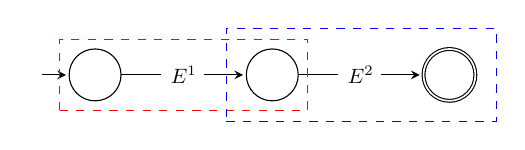
\begin{tikzpicture}[->,>=stealth,shorten >=1pt,auto,node distance=1.5 cm, scale = 0.75, transform shape,initial text={}]
  \node [initial, state] (0) {};
  \node [right of= 0] (1) {$E^1$};
  \node [state,right of= 1] (2) {};
  \node [right of= 2] (3) {$E^2$};
  \node [accepting, state,right of= 3] (4) {};

  \path[-] (0) edge node {} (1);
  \path[-] (2) edge node {} (3);

  \path[->] (1) edge node {} (2);
  \path[->] (3) edge node {} (4);

\node [draw=red, fit= (0) (2),dashed] {};
\node [draw=blue, fit= (2) (4),dashed,inner sep=0.25cm] {};
  
\end{tikzpicture}\end{center} \\
\hline
\begin{center}$E^1 + E^2$\end{center} &\begin{center} 
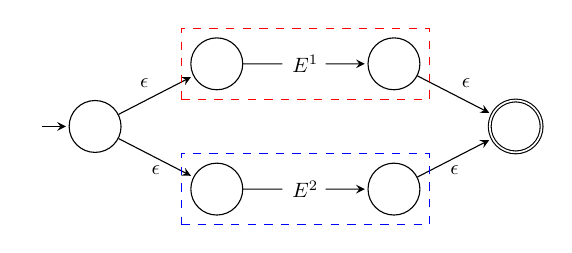
\begin{tikzpicture}[->,>=stealth,shorten >=1pt,auto,node distance=1.5 cm, scale = 0.75, transform shape,initial text={}]
  \node [initial, state] (0) {};
  \node [state,above right of=0,xshift=1cm] (1) {};
  \node [state,below right of=0,xshift=1cm] (2) {};
  \node [right of =1] (3) {$E^1$};
  \node [right of=2] (4) {$E^2$};
  \node [state, right of=3] (5) {};
  \node [state, right of=4] (6) {};
  \node [accepting,state,below right of=5,xshift=1cm] (7) {};

  \path[-] (1)edge node {} (3);
  \path[-] (2)edge node {} (4);

  \path[->] (0) edge node {$\epsilon$} (1);
  \path[->] (0) edge node[below] {$\epsilon$} (2);
  \path[->] (3) edge node {} (5);
  \path[->] (4) edge node {} (6);
  \path[->] (5) edge node {$\epsilon$} (7);
  \path[->] (6) edge node[below] {$\epsilon$} (7);


\node [draw=red, fit= (1) (5),dashed] {};
\node [draw=blue, fit= (2) (6),dashed] {};

\end{tikzpicture} \end{center} \\
\hline
\begin{center}$E^*$\end{center} &\begin{center} 
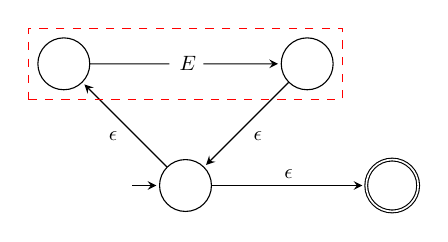
\begin{tikzpicture}[->,>=stealth,shorten >=1pt,auto,node distance=1.5 cm, scale = 0.75, transform shape,initial text={}]
  \node [initial, state] (0) {};
  \node [accepting,state,right of=0,xshift=2cm] (1) {};
  \node [state,above left of=0,xshift=-1cm,yshift=1cm] (2) {};
  \node [state,above right of=0,xshift=1cm,yshift=1cm] (3) {};
  \node [right of=2,xshift=0.60cm] (4) {$E$};

  \path[->] (0) edge node {$\epsilon$} (1);
  \path[->] (3) edge node {$\epsilon$} (0);
  \path[->] (0) edge node {$\epsilon$} (2);
  \path[->] (4) edge node {} (3);

  \path[-] (2) edge node {} (4);

\node [draw=red, fit= (2) (3),dashed] {};
\end{tikzpicture}
\end{center} \\
\hline
\end{tabular}
\label{tab:TNFA}
\end{table}
\newpage
\subsection{Simulating TNFA}\label{section_TNFA}
TNFA simulation adds an additional argument for amount of mismatches allowed. The stateset contains 4 tuples of $(Q,i,d,a)$ where i,d and a is a count of how many of each transition has been used. The $\epsilon-closure$ and $reachable$ functions are extended to allow for for a set of 4 tuples.
\begin{mydef} 
Given a 4 tuple containing a state and mismatch counters $S(s,i,d,a)$, and a mismatch type $M$, the $t$-$reachable$ of S is a 4 tuple with the state that is reachable following the tagged transtion of the mismatch type $M$ in $\Delta'$ and the mismatch counters, with the mismatch type increased by one.  
\end{mydef}
\begin{algorithm}[h!]
  \caption{TNFA simulation
    \label{tnfasim}}
  \begin{algorithmic}[1]
    \Require{$N$ is a TNFA and $s$ is a string,M is a 3-tuple of mismatches allowed}
    \Ensure{True if $s$ is accepted in $N$ with $M$ mismatches, False if $s$ is rejected in $N$}
    \Function{Simulation}{$N(Q,\Sigma,\Delta,q^s,q^a,\Delta'), s,M$}
      \Let{$stateset$}{$\{q^s,0,0,0\}$} 
      \For{{\bf each} symbol {\bf in} $s$}
        \If{$stateset = \emptyset$} 
            \State \Return{False}
        \EndIf
        \Let{$next$}{$\emptyset$}
        \Let{$states$}{$\epsilon$-closure($stateset$)}
        \Let{$next$}{$reachable(symbol,states)$}
        	\Let{$t\_next$}{$TNFA$-$reach(states,M)$}
          \Let{$stateset$}{$next \cup t\_next$}
      \EndFor
      \If{$q^a \in stateset$}
        \State \Return{True}
      \EndIf
      \State \Return{False}
    \EndFunction
  \end{algorithmic}
\end{algorithm}

\begin{algorithm}[h!]
  \caption{
    \label{tnfatrans}}
  \begin{algorithmic}[1]
    \Require{$states$ is a set of 4 tuples with a state q and mismatches occured, $M$  is a 3-tuple of mismatches allowed}
    \Ensure{A stateset with states that are reachable from $states$ using mismatches}
    \Function{$TNFA$-$reach$}{$states,M(ins,del,alt)$}
      \Let{$stateset$}{$\emptyset$} 
      \For{{\bf each} state(s,i,d,a) {\bf in} $states$}
        \Let{$stateset$}{$stateset \cup reachable(state)$}
        \If{$i < ins$}
        	\Let{$stateset$}{$stateset ~ \cup ~ (t$-$reachable(state,i)$}
        \EndIf
        \If{$d < del$}
        	\Let{$stateset$}{$stateset ~\cup ~ (t$-$reachable(state,d))$}
        \EndIf
        \If{$a < alt$}
        	\Let{$stateset$}{$stateset ~\cup~ (t$-$reachable(state,a))$}
        \EndIf
      \EndFor
      \State \Return{$stateset$}
    \EndFunction
  \end{algorithmic}
\end{algorithm}

\newpage


\begin{myex}
Given the RE $E= {\tt abc}^*{\tt d}$ the resulting TNFA N can be seen in Figure \ref{tnfa:simsuc}
\begin{figure}[H]
\begin{center}
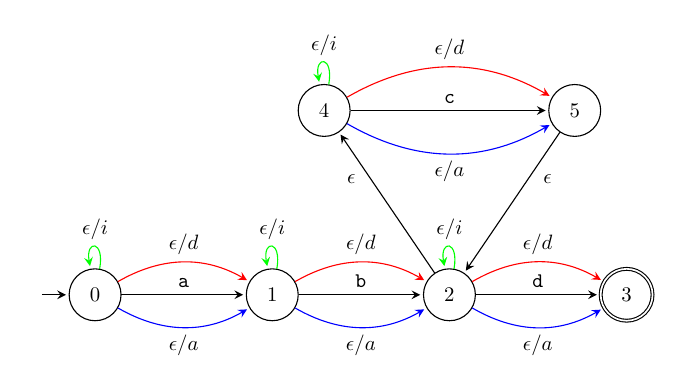
\begin{tikzpicture}[->,>=stealth,shorten >=1pt,auto,node distance=3 cm, scale = 0.75, transform shape,initial text={}]
  \node [initial, state] (0) {0};
  \node [state,right of=0] (1) {1};
  \node      [state,right of=1] (2) {2};
   \node     [accepting,state,right of=2] (3) {3};
    \node    [state,above left of=2,yshift=1cm] (4) {4};
    \node    [state,above right of=2,yshift=1cm] (5) {5};


   \path[->] (0) edge node {{\tt a}} (1)
         (1) edge node {{\tt b}} (2)
         (2) edge node {{\tt d}} (3)
           edge node [near end] {$\epsilon$} (4)
         (4) edge node {{\tt c}} (5)
         (5) edge node [near start] {$\epsilon$} (2);


  \path[->] (0) edge [color=green, in=100,out=80,loop] node [color=black, above] {$\epsilon/i$} (0);
  \path[->] (0) edge [color=red,bend left] node [color=black, above] {$\epsilon/d$} (1);
  \path[->] (0) edge [color=blue,bend right] node [color=black, below] {$\epsilon/a$} (1);


  \path[->] (1) edge [color=green, in=100,out=80,loop] node [color=black, above] {$\epsilon/i$} (1);
  \path[->] (1) edge [color=red,bend left] node [color=black, above] {$\epsilon/d$} (2);
  \path[->] (1) edge [color=blue,bend right] node [color=black, below] {$\epsilon/a$} (2);

  \path[->] (2) edge [color=green, in=100,out=80,loop] node [color=black, above] {$\epsilon/i$} (2);
  \path[->] (2) edge [color=red,bend left] node [color=black, above] {$\epsilon/d$} (3);
  \path[->] (2) edge [color=blue,bend right] node [color=black, below] {$\epsilon/a$} (3);

  \path[->] (4) edge [color=green, in=100,out=80,loop] node [color=black, above] {$\epsilon/i$} (4);
  \path[->] (4) edge [color=red,bend left] node [color=black, above] {$\epsilon/d$} (5);
  \path[->] (4) edge [color=blue,bend right] node [color=black, below] {$\epsilon/a$} (5);
\end{tikzpicture}
\end{center}
\caption{TNFA of expression $E = {\tt abc}^*{\tt d}$}
\label{tnfa:simsuc}
\end{figure}
We now want to see if the input string {\tt "abbdd"} is accepted in N allowing 1 insertion and 1 deletion. The initial stateset \{($q^s$,i,d,a)\} =\{(0,0,0,0)\}\\\\
\begin{table}[h!]
\small
\begin{tabular}{l l l}
\multicolumn{2}{l}{TNFASimulate(N,{\tt abbdd},(1,1,0)):}\\
symbol {\tt a}:& $\epsilon$-$closure$(\{(0,0,0,0)\})&=\{(0,0,0,0)\}\\
&$reachable$(\{(0,0,0,0)\},{\tt a})&=\{(1,0,0,0)\}\\
&$t$-$reachable$(\{(0,0,0,0)\},i)&=\{(0,1,0,0)\}\\
&$t$-$reachable$(\{(0,0,0,0)\},d)&=\{(1,0,1,0)\}\\
&$next\_stateset$&=\{(1,0,0,0),(0,1,0,0),(1,0,1,0)\}\\
\\
symbol {\tt b}:& $\epsilon$-$closure$(\{(1,0,0,0),(0,1,0,0),(1,0,1,0)\}) &=\{(1,0,0,0),(0,1,0,0),(1,0,1,0)\}\\
&$reachable$(\{(1,0,0,0),(0,1,0,0),(1,0,1,0)\},{\tt b})&=\{(2,0,0,0),(2,0,1,0)\}\\
&$t$-$reachable$(\{(1,0,0,0),(0,1,0,0),(1,0,1,0)\},i)&=\{(1,1,0,0),(1,1,1,0)\}\\
&$t$-$reachable$(\{(1,0,0,0),(0,1,0,0),(1,0,1,0)\},d)&=\{(2,0,1,0),(1,1,1,0)\}\\
&$next\_stateset$&=\{(2,0,0,0),(2,0,1,0),(1,1,0,0),(1,1,1,0)\}\\
\\ 
symbol {\tt b}:&$\epsilon$-$closure$(\{(2,0,0,0),(2,0,1,0),(1,1,0,0),(1,1,1,0)\})&=\{(2,0,0,0),(2,0,1,0),(1,1,0,0)\\
&&~~~,(1,1,1,0),(4,0,0,0),(4,0,1,0)\}\\
&$reachable$(\{(2,0,0,0),(2,0,1,0),(1,1,0,0),(1,1,1,0)&=\{(2,1,0,0),(2,1,1,0)\}\\
&~~~~~~~~~~~~~~,(4,0,0,0),(4,0,1,0)\},{\tt b})\\

&$t$-$reachable$(\{(2,0,0,0),(2,0,1,0),(1,1,0,0),(1,1,1,0)&=\{(2,1,0,0),(2,1,1,0),(4,1,0,0),(4,1,1,0)\}\\
&~~~~~~~~~~~~~~~~,(4,0,0,0),(4,0,1,0)\},i)\\

&$t-reachable$(\{(2,0,0,0),(2,0,1,0),(1,1,0,0),(1,1,1,0)&=\{(3,0,1,0),(3,1,1,0),(5,0,1,0)\}\\
&~~~~~~~~~~~~~~~~,(4,0,0,0),(4,0,1,0)\},d)\\

&$next\_stateset$&=\{(2,1,0,0),(2,1,1,0),(3,0,1,0),(3,1,1,0)\\
&&~~~,(4,1,0,0),(4,1,1,0),(5,0,1,0)\}\\
\\
symbol {\tt d}:&$\epsilon$-$closure$(\{(2,1,0,0),(2,1,1,0),(3,0,1,0),(3,1,1,0)&=\{(2,1,0,0),(2,0,1,0),(2,1,1,0),(3,0,1,0),(3,1,1,0)\\
&~~~~~~~~~~~~~~,(4,1,0,0),(4,1,1,0),(5,0,1,0)\}&~~~,(4,1,0,0),(4,0,1,0),(4,1,1,0),(5,0,1,0)\}\\
&$reachable$(\{(2,1,0,0),(2,0,1,0),(2,1,1,0),(3,0,1,0),(3,1,1,0)&=\{(3,1,0,0),(3,0,1,0),(3,1,1,0)\}\\
&~~~~~~~~~~~~~~,(4,1,0,0),(4,0,1,0),(4,1,1,0),(5,0,1,0)\},{\tt d})\\

&$t$-$reachable$(\{(2,1,0,0),(2,0,1,0),(2,1,1,0),(3,0,1,0),(3,1,1,0)&=\{(3,1,1,0),(5,1,1,0)\}\\
&~~~~~~~~~~~~~~~~,(4,1,0,0),(4,0,1,0),(4,1,1,0),(5,0,1,0)\},i)\\

&$t$-$reachable$(\{(2,1,0,0),(2,0,1,0),(2,1,1,0),(3,0,1,0),(3,1,1,0)&=\{(3,1,1,0),(5,1,1,0)\}\\
&~~~~~~~~~~~~~~~~,(4,1,0,0),(4,0,1,0),(4,1,1,0),(5,0,1,0)\},d)\\
&$next\_stateset$&=\{(3,1,0,0),(3,0,1,0),(3,1,1,0),(5,1,1,0)\}\\
\\
symbol {\tt d}:&$\epsilon$-$closure$(\{(3,1,0,0),(3,0,1,0),(3,1,1,0),(5,1,1,0)\})&=\{(3,1,0,0),(3,0,1,0),(3,1,1,0),(5,1,1,0)\\
&&~~~,(2,1,1,0),(4,1,1,0)\}\\
&$reachable$(\{(3,1,0,0),(3,0,1,0),(3,1,1,0),(5,1,1,0)&=\{3,1,1,0\}\\
&~~~~~~~~~~~~~~,(2,1,1,0),(4,1,1,0)\},{\tt d})\\
&$t$-$reachable$(\{(3,1,0,0),(3,0,1,0),(3,1,1,0),(5,1,1,0)&=$\emptyset$\\
&~~~~~~~~~~~~~,(2,1,1,0),(4,1,1,0)\},i)\\
&$t$-$reachable$(\{(3,1,0,0),(3,0,1,0),(3,1,1,0),(5,1,1,0)&=$\emptyset$\\
&~~~~~~~~~~~~~,(2,1,1,0),(4,1,1,0)\},d)\\
&$final\_stateset$&=\{3,1,1,0\}
\end{tabular}
\end{table}\\
The string {\tt "abbdd"} is accepted, since $q^a\in final\_stateset$, which have 1 insertion and 1 deletion.
\end{myex}
\begin{myex}
Given the RE $E={\tt abbca}$ the TNFA $N$ of $E$ is seen in Figure \ref{tnfa:simfail}.
\begin{figure}[h!]
\begin{center}
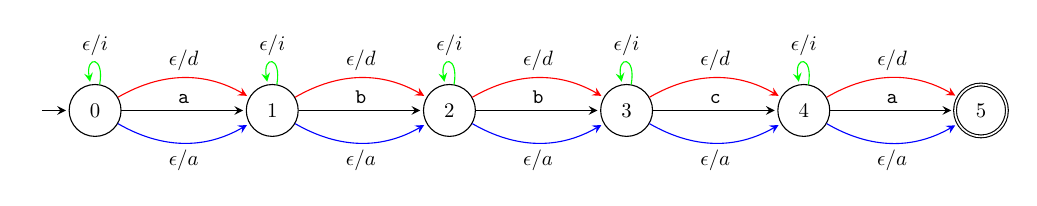
\begin{tikzpicture}[->,>=stealth,shorten >=1pt,auto,node distance=3 cm, scale = 0.75, transform shape,initial text={}]
  \node [initial, state] (0) {0};
  \node [state,right of=0] (1) {1};
  \node      [state,right of=1] (2) {2};
   \node     [state,right of=2] (3) {3};
   \node     [state,right of=3] (4) {4};
   \node     [accepting,state,right of=4] (5) {5};


   \path[->] (0) edge node {{\tt a}} (1)
         (1) edge node {{\tt b}} (2)
         (2) edge node {{\tt b}} (3)
         (3) edge node {{\tt c}} (4)
         (4) edge node {{\tt a}} (5);


  \path[->] (0) edge [color=green, in=100,out=80,loop] node [color=black, above] {$\epsilon/i$} (0);
  \path[->] (0) edge [color=red,bend left] node [color=black, above] {$\epsilon/d$} (1);
  \path[->] (0) edge [color=blue,bend right] node [color=black, below] {$\epsilon/a$} (1);


  \path[->] (1) edge [color=green, in=100,out=80,loop] node [color=black, above] {$\epsilon/i$} (1);
  \path[->] (1) edge [color=red,bend left] node [color=black, above] {$\epsilon/d$} (2);
  \path[->] (1) edge [color=blue,bend right] node [color=black, below] {$\epsilon/a$} (2);

  \path[->] (2) edge [color=green, in=100,out=80,loop] node [color=black, above] {$\epsilon/i$} (2);
  \path[->] (2) edge [color=red,bend left] node [color=black, above] {$\epsilon/d$} (3);
  \path[->] (2) edge [color=blue,bend right] node [color=black, below] {$\epsilon/a$} (3);

  \path[->] (3) edge [color=green, in=100,out=80,loop] node [color=black, above] {$\epsilon/i$} (3);
  \path[->] (3) edge [color=red,bend left] node [color=black, above] {$\epsilon/d$} (4);
  \path[->] (3) edge [color=blue,bend right] node [color=black, below] {$\epsilon/a$} (4);

  \path[->] (4) edge [color=green, in=100,out=80,loop] node [color=black, above] {$\epsilon/i$} (4);
  \path[->] (4) edge [color=red,bend left] node [color=black, above] {$\epsilon/d$} (5);
  \path[->] (4) edge [color=blue,bend right] node [color=black, below] {$\epsilon/a$} (5);
\end{tikzpicture}
\end{center}
\caption{TNFA of expression $E = {\tt abbca}$}
\label{tnfa:simfail}
\end{figure}
We now want to see the string {\tt "abccec"} is accepted into $N$ given the initial stateset \{(0,0,0,0)\} and allowing 1 insertion and 1 alternation.\\
\begin{table}[h!]
\small
\begin{tabular}{l l l}
\multicolumn{2}{l}{TNFASimulate(N,{\tt abccec},(1,0,1)):}\\
symbol {\tt a}:& $\epsilon$-$closure$(\{(0,0,0,0)\})&=\{(0,0,0,0)\}\\
&$reachable$(\{(0,0,0,0)\},{\tt a})&=\{(1,0,0,0)\}\\
&$t$-$reachable$(\{(0,0,0,0)\},i)&=\{(0,1,0,0)\}\\
&$t$-$reachable$(\{(0,0,0,0)\},a)&=\{(1,0,0,1)\}\\
&$next\_stateset$&=\{(1,0,0,0),(0,1,0,0),(1,0,0,1)\}\\
\\
symbol {\tt b}:& $\epsilon$-$closure$(\{(1,0,0,0),(0,1,0,0),(1,0,0,1)\})&=\{(1,0,0,0),(0,1,0,0),(1,0,0,1)\}\\
&$reachable$(\{(1,0,0,0),(0,1,0,0),(1,0,0,1)\},{\tt b})&=\{(2,0,0,0),(2,0,0,1)\}\\
&$t$-$reachable$(\{(1,0,0,0),(0,1,0,0),(1,0,0,1)\},i)&=\{(1,1,0,0),(1,1,0,1)\}\\
&$t$-$reachable$(\{(1,0,0,0),(0,1,0,0),(1,0,0,1)\},a)&=\{(1,1,0,1),(2,0,0,1)\}\\
&$next\_stateset$&=\{(1,1,0,0),(1,1,0,1),(2,0,0,0),(2,0,0,1)\}\\
\\
symbol {\tt c}:& $\epsilon$-$closure$(\{(1,1,0,0),(1,1,0,1),(2,0,0,0),(2,0,0,1)\})&=\{(1,1,0,0),(1,1,0,1),(2,0,0,0),(2,0,0,1)\}\\
&$reachable$(\{(1,1,0,0),(1,1,0,1),(2,0,0,0),(2,0,0,1)\},{\tt c})&=$\emptyset$\\
&$t$-$reachable$(\{(1,1,0,0),(1,1,0,1),(2,0,0,0),(2,0,0,1)\},i)&=\{(2,1,0,0),(2,1,0,1)\}\\
&$t$-$reachable$(\{(1,1,0,0),(1,1,0,1),(2,0,0,0),(2,0,0,1)\},a)&=\{(2,1,0,1),(3,0,0,1)\}\\
&$next\_stateset$&=\{(2,1,0,0),(2,1,0,1),(3,0,0,1)\}\\
\\
symbol {\tt c}:& $\epsilon$-$closure$(\{(2,1,0,0),(2,1,0,1),(3,0,0,1)\})&=\{(2,1,0,0),(2,1,0,1),(3,0,0,1)\}\\
&$reachable$(\{(2,1,0,0),(2,1,0,1),(3,0,0,1)\},{\tt c})&=\{(4,0,0,1)\}\\
&$t$-$reachable$(\{(2,1,0,0),(2,1,0,1),(3,0,0,1)\},i)&=\{(3,1,0,1)\}\\
&$t$-$reachable$(\{(2,1,0,0),(2,1,0,1),(3,0,0,1)\},a)&=\{(3,1,0,1)\}\\
&$next\_stateset$&=\{(3,1,0,1),(4,0,0,1)\}\\
\\
symbol {\tt e}:& $\epsilon$-$closure$(\{(3,1,0,1),(4,0,0,1)\})&=\{(3,1,0,1),(4,0,0,1)\}\\
&$reachable$(\{(3,1,0,1),(4,0,0,1)\},{\tt e})&=$\emptyset$\\
&$t$-$reachable$(\{(3,1,0,1),(4,0,0,1)\},i)&=\{(4,1,0,1)\}\\
&$t$-$reachable$(\{(3,1,0,1),(4,0,0,1)\},a)&=$\emptyset$\\
&$next\_stateset$&=\{(4,1,0,1)\}\\
\\
symbol {\tt c}:& $\epsilon$-$closure$(\{(4,1,0,1)\})&=\{(4,1,0,1)\}\\
&$reachable$(\{(4,1,0,1)\},{\tt c})&=$\emptyset$\\
&$t$-$reachable$(\{(4,1,0,1)\},i)&=$\emptyset$\\
&$t$-$reachable$(\{(4,1,0,1)\},a)&=$\emptyset$\\
&$next\_stateset$&=$\emptyset$\\
\\
\end{tabular}
\end{table}\\\\\\
At the end of reading input $\emptyset$ is found, the string {\tt abccec} is not accepted into $N$.
\end{myex}
%Simulation of NFA

\documentclass[11pt,twoside,a4paper]{article}
\usepackage{pbox}
\usepackage{amsthm}
\newtheorem{definition}{Definition}
\newtheorem{example}{Example}
\begin{document}
\subsection{Scan\_For\_Matches}
Scan\_for\_matches is a string-searching tool created by Ross Overbeek, David 
Joerg and Morgan Price in C which searches through FASTA text files. Users specify 
what they wish to search for by defining a pattern, and scan\_for\_matches 
returns all matches that corresponds to the specified pattern.
\begin{definition}\label{patd}
A pattern is defined as follows:\\
\begin{tabular}{|r|l|}
\hline
{\tt ACUG}&Match the sequence ACUG\\
\hline
{\tt 1...5}&Match 1 to 5 characters\\
\hline
{\tt 3...3}&Match exactly 3 characters\\
\hline
{\tt p1=1...5}&Match 1 to 5 characters, and call the sequence p1\\
\hline
{\tt p1 $|$ p2}&Match either p1 or p2\\
\hline
{\tt p1[1,0,0]}&Match p1, allowing for one mismatch\\
\hline
{\tt p1[0,1,0]}&Match p1, allowing for one deletion\\
\hline
{\tt p1[0,0,1]}&Match p1, allowing for one insertion\\
\hline
{\tt length(p1+p2) $<$ 5}&The combined length of p1 and p2 must not exceed 4\\
\hline
{\tt r1=\{AB, BA\}}&\pbox{20cm}{Create a pattern rule where A is the complement of B, \\and B is the complement of A, and call it r1}\\
\hline
{\tt $<$p1}&Match the reverse of p1\\
\hline
{\tt \textasciitilde p1}&\pbox{20cm}{Match the reverse complement of p1 using the G-C, \\C-G, A-T and T-A pairing rule}\\
\hline
{\tt r1\textasciitilde p1}&\pbox{20cm}{Match the reverse complement of p1 using r1 rules}\\
\hline
{\tt \textasciicircum ~p1}&\pbox{20cm}{Match only p1 if it is at the start of a string}\\
\hline
{\tt p1 \$}&Match only p1 if it is at the end of a string\\
\hline
\end{tabular}
\end{definition}

\begin{definition}\label{patc}
Let {\tt E} be any pattern that's in the alphabet $\Sigma$ as defined in Definition \ref{patd}. 
Let $\epsilon$ be the empty string.
Let {\tt A} be a string that we are processing to see if the pattern is valid.
A pattern may then be constructed as such: \begin{center}
{\tt A = A' A | $\epsilon$}\\
{\tt A' = E}\end{center}
\end{definition}
Definition \ref{patc} states that a pattern may be any combination of the alphabet 
defined in definition \ref{patd}.
Using these patterns, it is possible to make very specific or very broad 
searches in a text file. 

\begin{example}
Say we want to write a pattern that finds the sequence {\tt GUUC}, allowing 
one mismatch, followed by a random sequence which has a length between 3 and 5, 
followed by the reverse complement of the first sequence that we found. We can 
then write this as \begin{center}
{\tt p1=GUUC[1,0,0] 3...5 \textasciitilde p1}
\end{center}
\end{example}

\end{document}

%implementation
%\section{Method}
%\newpage
\documentclass[11pt,twoside,a4paper]{article}
\newtheorem{mydef}{Definition}
\newtheorem{myex}{Example}
\begin{document}





\end{document}

\newpage
\section{Our Implementation}
Having defined an algorithm in Section~\ref{sec:tnfa}, we wished to construct a simple program based on TNFA, which would pattern-match data allowing for mismatches.

% Torbens noter kræver begrundelse for beslutninger, hvorfor bruger vi C++
We wrote a simple program in C++, in order to ensure strict control of the types and behavior of our code. We named the program TNFA Pattern-Matcher (TPaMa). TPaMa is able to create an NFA from a RE, as described in Section~\ref{RA_TO_NFA}, by supporting a series of RE symbols along with concatenation of characters.
% An example of a TFNA from a RE could be RE "(GAT)+" which would produce a structure as shown in Figure~\ref{fig:gat}

%\begin{figure}[h!]
%\centering
%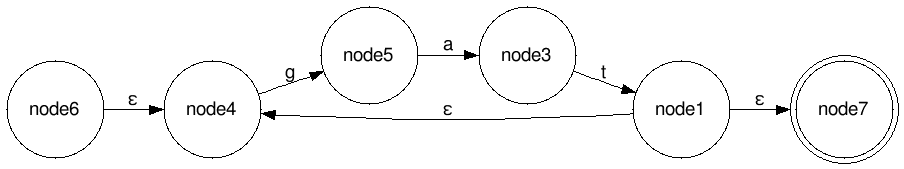
\includegraphics[width=0.5\textwidth]{lib/gat.png}
%\caption{Example of how TPaMa constructs a TNFA from RE (GAT)+}
%\label{fig:gat}
%\end{figure}

Currently the search implementation of TPaMa only support simple patterns such as "GAT", which does not cause any $\epsilon$-transitions to be constructed. This choice was made, so we could focus on the performance of mismatching while giving support to the most crucial part of pattern-matching.

This also meant that determining reachable states, as mentioned in Algorithm~\ref{tnfasim} \&~\ref{tnfatrans}, is rather straightforward, as there's only up to one possible next state for every state (zero for the final state). 

To handle mismatching, recall Table~\ref{nfac}:

%\begin{table}[h]
\begin{tabular}{*{2}{m{0.4\textwidth}}}
\begin{center}$a$\end{center} &\begin{center}
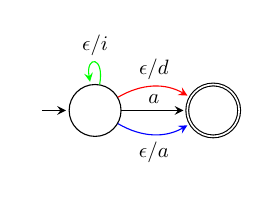
\begin{tikzpicture}[->,>=stealth,shorten >=1pt,auto,node distance=2 cm, scale = 0.75, transform shape,initial text={}]
  \node [initial, state] (0) {};
  \node [accepting,state, right of=0] (1) {};

  \path[->] (0) edge node [above] {$a$} (1);
  \path[->] (0) edge [color=green, in=100,out=80,loop] node [color=black, above] {$\epsilon/i$} (0);
  \path[->] (0) edge [color=red,bend left] node [color=black, above] {$\epsilon/d$} (1);

  \path[->] (0) edge [color=blue,bend right] node [color=black, below] {$\epsilon/a$} (1);
\end{tikzpicture}\end{center}\\
\end{tabular}
%\end{table}

There's three different types of mismatches. Instead of having three types of transitions, as the theory call for, in the simulation we solve this by having three counters in each state, one for each type of mismatch (insertions, alternation and deletion), keeping track of the remaining number of mismatches allowed in the match. Whenever a match can not be made, for each mismatch counter with a positive value, a new state is created corresponding to the transitions above; alternations and deletions both advance the state to the next reachable, while insertions remain in the same state in the TNFA, the corresponding mismatch counter is decreased and the pattern-matching continues.

For every state in the stateset, at some point it will either match the final state of the TFNA at which point a match is printed, or a state will not be able to match, even with mismatches, at which point it will be erased from the stateset. This continues until all data has been checked, at which point the TPaMa terminates.
\section{Experimental Results \& Tests}
Using our implementation, TRE and scan\_for\_matches, we were able to do some benchmarking in order to compare performances.

For this a virtual machine is created, using Oracle VirtualBox\footnote{virtualbox.org}. The machine running the virtualbox is running Windows 8.1 Pro x64 of an SSD, with 8,00 GB RAM, an AMD FX 4300 Quad-Core Processor 3.80 GHz, of which 1 core and 4096MB RAM was given to the virtual machine, which would run Ubuntu 14.04.2 LTS 64 bit.

\begin{wrapfigure}{r}{0.5\linewidth}
\centering
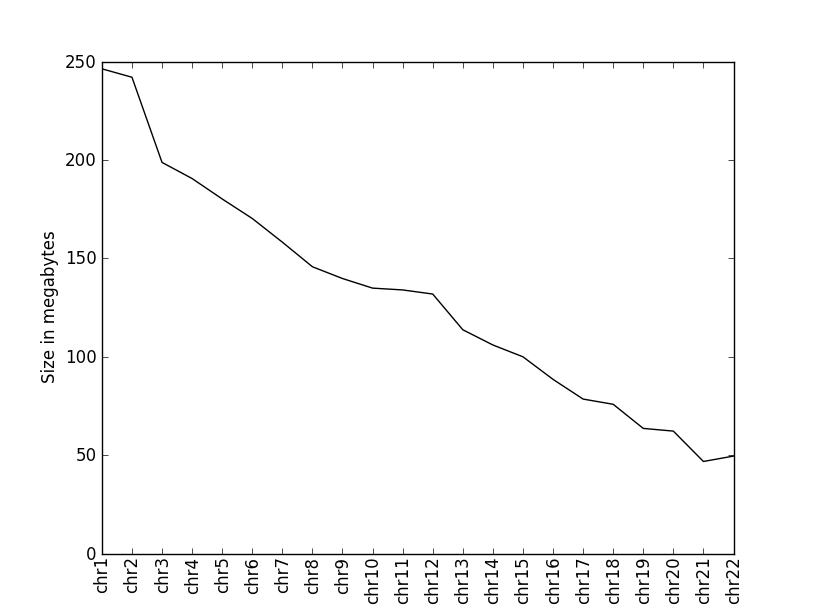
\includegraphics[width=0.3\textwidth]{Benchmarking/size.png}
\caption{Plot of sample files used for benchmarking, these files range from 246.3 Megabytes to 46.8 Megabytes in size}
\label{fig:size}
\end{wrapfigure}

For the benchmarking some data was required, figure~\ref{fig:size} shows a series of fasta files, these files include nucleotide sequences, which all differ in size, decreasing from chr1 to chr22. These fasta files are the  kind of data which scan\_for\_matches are expected to run, and thus excellent for benchmark testing, it's worth noting however, that each of these files are 50 characters long, as TRE matches searches through lines separately, and longer or shorter line sizes might affect the performance of TRE, this was not tested.

For testing, a suitable pattern is required. As our implementation has primarily been focused on supporting insertion, deletion and mutation on a sequence, a simple RNA sequence $TGCAAGCGTTAAT$ with variable insertions is chosen as the search pattern.

Each test would be executed on each of the mentioned fasta files a total of 10 times, given an average runtime which was used in the following results.

\begin{figure}[h!]
\centering
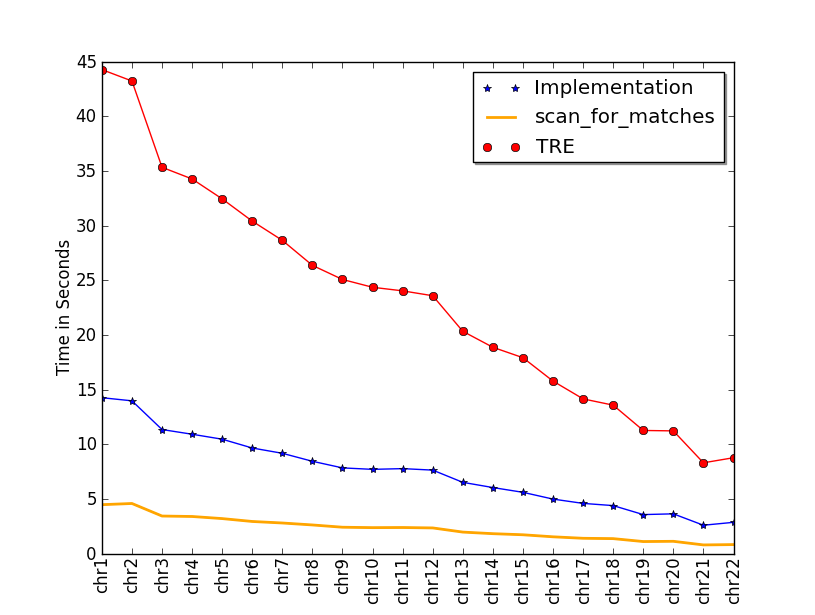
\includegraphics[width=0.5\textwidth]{Benchmarking/0miss.png}
\caption{Running time of search through fasta files mentioned in figure~\ref{fig:size} looking for pattern TGCAAGCGTTAAT with no missmatches}
\label{fig:0miss}
\end{figure}

First test was to see the runtime of each program, having no missmatches in the mentioned sequence RNA $TGCAAGCGTTAAT$, figure~\ref{fig:0miss} displays the results, and its clear to see that scan\_for\_matches is faster than both our implementation and TRE, and that all three programs have a decreased runtime as the data sizes lowers.

\begin{figure}[h!]
\begin{minipage}[b]{0.5\linewidth}
\centering
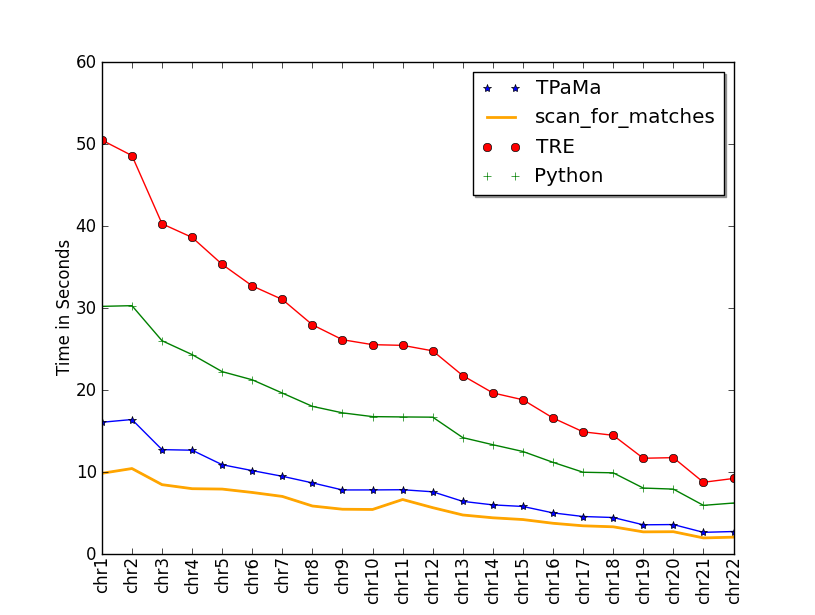
\includegraphics[width=0.8\textwidth]{Benchmarking/1ins.png}
\caption{Running time of search through fasta files mentioned in figure~\ref{fig:size},  allowing one insertions on pattern TGCAAGCGTTAAT}
\label{fig:ins1}
\end{minipage}
\hspace{0.25cm}
\begin{minipage}[b]{0.5\linewidth}
\centering
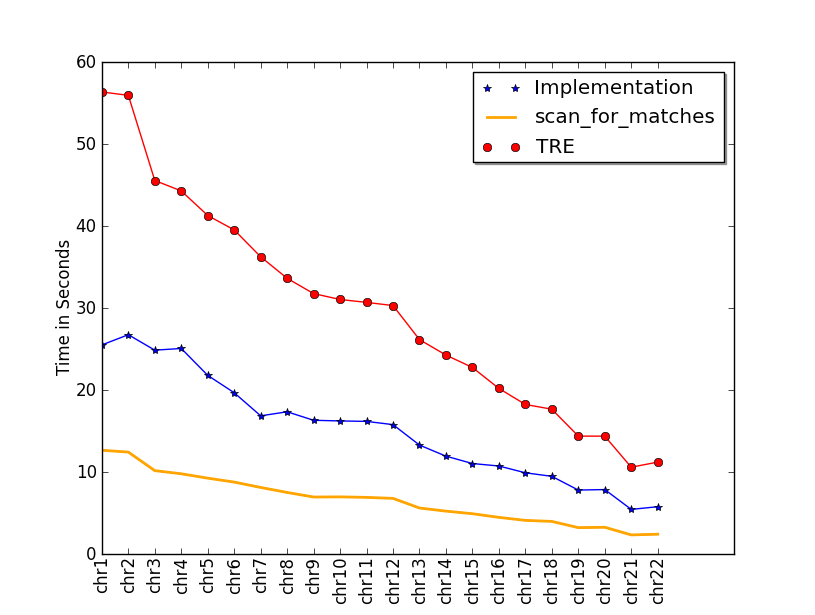
\includegraphics[width=0.8\textwidth]{Benchmarking/2ins.png}
\caption{Running time of search through fasta files mentioned in figure~\ref{fig:size},  allowing two insertions on pattern TGCAAGCGTTAAT}
\label{fig:ins2}
\end{minipage}
\end{figure}


From figure~\ref{fig:ins1} its visible that there's an increase in the runtime for scan\_for\_matches when adding an insertion to its pattern, and while both our implementation and TRE also has an increased runtime, it's not to the same scale as scan\_for\_matches.

Next test was to see the runtime of two insertions instead of one. Looking at figure~\ref{fig:ins2} scan\_for\_matches did increase its runtime slightly compared to figure~\ref{fig:ins1}, but the second insertion really affected our implementation, resulting in it running at about half the same speed of TRE.  And while TRE also had its runtime slightly increased, it's almost unchanged from one insertion.

\begin{figure}[h!]
\centering
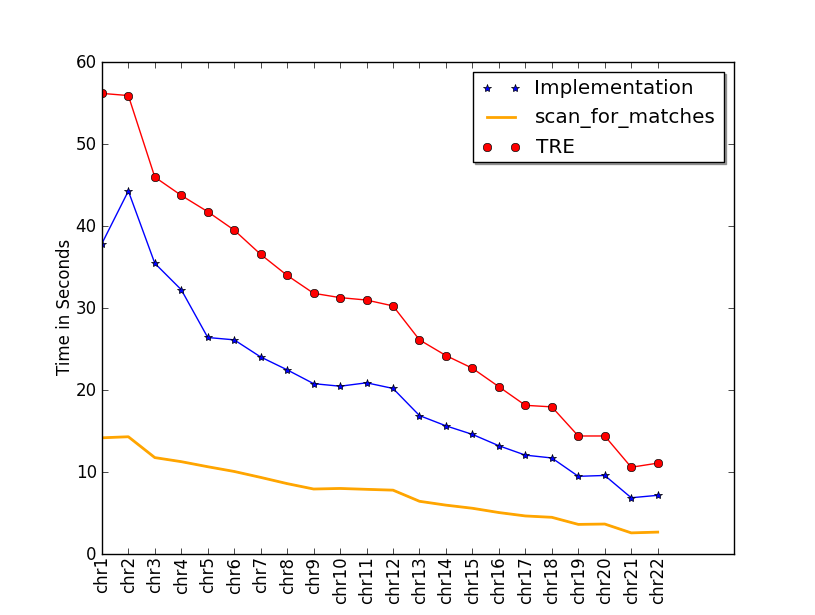
\includegraphics[width=0.5\textwidth]{Benchmarking/3ins.png}
\caption{Running time of search through fasta files mentioned in figure~\ref{fig:size},  allowing three insertions on pattern TGCAAGCGTTAAT}
\label{fig:ins3}
\end{figure}
Testing with three insertions, figure~\ref{fig:ins3} shows that once again our implementation had the worst increase in time compared to the two other options, almost reaching the same runtime as TRE.


From these three tests its clear to see that our implementation has a problem with increasing number of insertions. Increasing its runtime at a much higher rate than both scan\_for\_matches and TRE, from this we can conclude that our current implementation has a major flaw somewhere, should it be used with more advanced patterns. 
\\
~

Another interesting thing to test for was the number of hits when searching the files, in table~\ref{tab:hits} the number of hits which came up when searching on file chr1.fa are shown.

\begin{table}[h!]
\centering
\begin{tabular}{ l | c c r }
& 1 insertion & 2 insertions & 3 insertions\\
\hline
Our implementation& 5 &  47 & 235 \\
TRE& 1 & 19 & 76 \\
scan\_for\_matches & 5 & 43  & 192 \\
\end{tabular}
\caption{Number of hits in fasta file chr1, using the mentioned benchmark tests.}
\label{tab:hits}
\end{table}

The primary reason for our implementation to get more results than scan\_for\_matches is that our implementation finds every single match in the file, including overlapping matches, while scan\_for\_matches, by default, only finds matches which does not overlap. TRE has the major disadvantage here that it doesn't match across newlines, causing it to miss a lot of matches.



%alternative soloutions
\section{Alternative soloutions}
\subsection{Forming patterns using Regular expressions}
The initial goal of this project was to use regular expressions to match the sequences. The problem of only using regular expressions, is the amount of patterns explode in size when adding mismatching. Following is a description of how many patterns are formed from a pattern of length $n$. When a new pattern is formed, it constructs them into 1 regular expression using the alternation operator separating each of the new expressions. 

Mutations are done by having a character replaced by a wildcard. This is done for every character in the pattern. When adding multiple mutations, characters which are already wildcards are not changed. The formula for the amount of patterns formed from mutations is the number of combinations that can be formed from the amount of mutations in $t$. This is the binomial coefficient\footnote{\url{http://en.wikipedia.org/wiki/Binomial_coefficient}}. 

An insertion is a wildcard added between the characters in the pattern, so for each pattern $n-1$ new patterns occur.

A deletion is removing a character from the pattern. It is not allowed to remove a character next to an insertion, as this cannot occur in RNA and DNA strings. Given multiple insertions, they will be spread out throughout the pattern in most cases, so an approximation of how many patterns formed would be $(n - insertions * 2)$.

The final formula looks like ${n \choose m}*(n-1)*(n-i*2)$, where $n$ is the length of the string, $m$ is amount of mutations and i is amount of insertions.

\begin{myex}\label{altreg}
Given a pattern of size 30, with 2 mutations, 1 deletion, 1 insertion. It would produce the following amount of patterns: \\
\begin{center}
\text{After mutation:} $~{30 \choose 2} = 435$\\
\text{After insertion:} $435 * (30-1) = 12615$\\
After~Deletion:~$12615*(30-2) = 353220$
\end{center}
\end{myex}

As shown in example \ref{altreg}, the amount of patterns formed from using regular expressions could be too large for a regular expression matcher to find in a reasonable time. 

\subsection{Preprocessing data}
Preprocessing data gives certain advantages, as it allows for faster lookups into the string that is being searched on. With a structure like suffix trees\footnote{\url{http://en.wikipedia.org/wiki/Suffix_tree}}, to store the location of all the substrings. It would be possible to do lookups in constant time given the correct choice of data structures. This would allow using the large regular expressions with mismatches to be run in a reasonable time.
The disadvantage of preprocessing data, is the time it takes to construct an indexed structure of the string, and it may produce a tree larger than the original string, which could be an issue in some of the larger data files which are several GB in size. If the file have to be reused many times, it may be justified to create one. 

% READ ME!!!!!!!
% Det der står i scan-for-matches omtaler et alfabet og et sprog, dette er først beskrevet i Theory/re.tex, derfor skal det ind bagefter
% HVIS vi skal beskrive scan-for-matches først, kan vi nævne at det findes et værktøj, og hvad det bruges til, men den måde det står beskrevet pt, funker ikke.
%related works, SFM TRE
% \READ ME
%\section{Method}
%
%experimental results
%\section{Conclusion}
\newpage
\nocite{*}
\bibliographystyle{unsrt}
\bibliography{./References/references}
\end{document}
